%priprava posamezne ure
%tukaj zaporedoma napisemo{st. zaporedne ure}{datum}{naslov}{poglavje}{oblika dela}{pripomocki}
\begin{priprava}{}{}{Integral}{Določeni integral}{frontalna}{tabla}

\didopomba{Začnemo z nečim, kar na prvi pogled nima veze z integralom.}

\naslov{Geometrijski pomen}

Koliko je ploščina območja, ki ga funkcija $ f(x) = x - 1 $ na intervalu $ [2, 4] $ oklepa z $ x $-osjo? \didopomba{Izračunamo iz slikce. Nato pa zakoplicirajmo.}

\didopomba{Narišeš dovolj vijugasto funkcijo $ f(x) $, nenegativno na intervalu $ [a, b] $, zdaj pa nas zanima ploščina pod njenim grafom. Dobimo jo z razdelitvijo območja na znane like, mi vzamemo pravokotnike, ampak s kakšno višino? Ploščino lahko omejimo z zgornjo in spodnjo vsoto (razloži, kaj je to, čim manj oznak!), če delamo vedno drobnejše delitve, pa pridemo prav do te ploščine: aplet v Geogebri \\(https://www.geogebra.org/m/Fv6t696j, tega si ne rabijo pisat!)}

\begin{figure*}[h!]
    \centering
    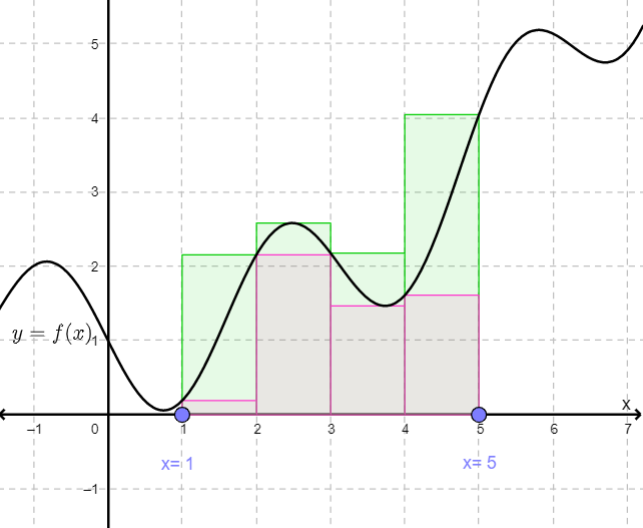
\includegraphics[width=6cm]{slike/vsote1.png}
    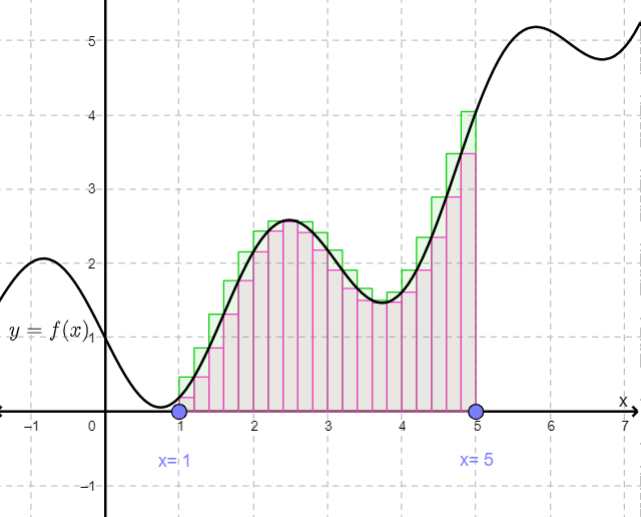
\includegraphics[width=6cm]{slike/vsote2.png}
\end{figure*}

\didopomba{Iz animacije vidimo, da je ploščina območja omejena od spodaj s spodnjo vsoto, od zgoraj pa z zgornjo vsoto. In to ne glede na število delilnih točk. Tako se vidi, da se vsoti približujeta ploščini oz. nekemu številu, ki ga imenujemo:}


\textcolor{rdeca}{Določeni integral $ \int_a^b f(x) dx $ je enak ploščini lika, ki je omejen z grafom funkcije $ f $, $ x $-osjo ter premicama $ x = a $ in $ x = b $.} Pogoj: $ f (x) $ je zvezna in na $ [a, b] $ nenegativna.

$ a $ imenujemo \emph{spodnja meja} integrala, $ b $ pa \emph{zgornja meja}.

\didopomba{Zraven podobna slikica, kjer je označen pravokotnik s širino $ dx $ in višino $ f(x) $ (pač integral je izlimitirana vsota ...)
Poudari, da je dol. integral število (ne pa funkcija)! Zaenkrat ga še ne znamo izračunati, še pride}

\didopomba{Narišeš dve slikci, eno pod drugo. Na zgornji je graf nad $ x $-osjo, na drugi pa pod. Obakrat naj bo označena ploščina $ S $. Čim manj pisanja.}
\begin{itemize}
    \item (slikca s pozitivno funkcijo) $ \int_a^b f(x) dx $ = $ S_1 $
    \item (slikca z negativno funkcijo) $ \int_a^b f(x) dx $ = $ - S_2  \rightarrow \text{ ploščina } = |\int_a^b f(x) dx| $
\end{itemize}
Kaj pa, če je na $ [a, b] $ funkcija malo pozitivna, malo negativna? \didopomba{Slikca [a, c, b] interval, najprej pozitivna, nato negativna. S = S1 + S2 = prvi integral - drugi integral. Oziroma, celoten integral = vsota dveh podintegralov = prva ploščina - druga ploščina}

\newpage

Kratka vaja \vaje{(npr. slikco s polinomom z znanimi ploščinami, računaš le po eno območje naenkrat, pač enkrat bo +, enkrat -)}, potem pa še nekaj logičnih lastnosti \didopomba{sledijo iz ploščine (lahko zraven skice), se jih tudi preveri, ko spoznajo N-L formulo}:

\begin{itemize}
    \item $ \int_a^a f(x) dx = 0 $
    \item $ \int_a^c f(x) dx + \int_c^b f(x) dx = \int_a^b f(x) dx $, kjer je $ c \in [a, b] $
    \item $ \int_a^b f(x) dx = - \int_b^a f(x) dx $ \didopomba{To je bolj dogovor ...}
    \item $ \int_a^b c \cdot f(x) dx = c \cdot \int_a^b f(x) dx $
    \item $\int_a^b (f(x) + g(x)) dx = \int_a^b f(x) dx + \int_a^b g(x) dx $
    \item Izrek o povprečni vrednosti \didopomba{Območje na $ [a, b] $ deformiramo v pravokotnik s širino $ b - a $ (SLIKA!!). Koliko je višina? Ker sta ploščini enaki, velja $ \int_a^b f(x) dx = (b-a)p \rightarrow $}: $ p = \frac{1}{b - a} \int_a^b f(x) dx $
\end{itemize}

\vaje{
Vaje:
\begin{itemize}
    \item Lahko naloge - funckije z znano ploščino (jo znaš razbrati iz grafa, kakšne premice, absolutno, krožnice ...), najprej na enem območju, pozitivno/negativno, nato malo pozitivno in malo negativno
    \item funkcije, kjer se ploščine odštejejo v 0 (npr. lihe funkcije, $ \int_0^{2\pi} \sin x dx $)
    \item sode funkcije na simetričnem intervalu $ [-a, a] $ -- lahko integriraš po $ [0, a] $ in podvojiš! (včasih je to enostavneje, saj vstavljaš v eno mejo 0)
    \item valovita funkcija z odsekoma znanimi ploščinami (ampak neznanim predpisom) in morajo izračunati določeni integral na različnih intervalih, pa 2.f(x), pa -f(x), |f(x)| ipd.
    \item Oceni ploščino funkcije (npr. na [0, 2], min = 1 in max = 2 -> ploščina je med 2 in 4. Nato jo še izračunamo.) ALI npr. Za integral $ \int_e^{e^2} \ln x dx $ ugotovi, ali je večji od 2, ali je večji od 30. \didopomba{Naj sami razmislijo, kako se tega lotiti.}
\end{itemize}
}
 
Zdaj pa nam že malo nagaja, ker ne znamo izračunati določenega integrala ...

\naslov{Newton-Leibnizova formula}

\didopomba{Za začetek ponoviš nedoločen integral. Potema pa kar poveš formulo, zgodovinsko ozadje?}

Nedoločen integral: $ \int f(x) dx = F(x) + c, (F(x) + c)' = f(x) $

Določen integral: \textcolor{rdeca}{$ \int_a^b f(x) = F(x) |_a^b = F(a) - F(b) $ (N-L formula)}
\didopomba{Oznako $ F(x)|_a^b $ napiši na koncu (pustiš prazen prostor). Pojasni, zakaj tu ni konstante.}

\didopomba{Dokaz formule, če se ti zdi. Jih vprašaš, koliko jih zanima. Če se odločite za dokaz, ga ni treba pisat. Ideja: $ G(x) = \int_a^x f(t) dt $ je nedoločen integral za $ f $ ($ G'(x) = f(x) $ preko limite), torej $ G(x) = F(x) + c $. Velja $ G(a) = 0 = F(a) + c \rightarrow G(x) = F(x) - F(a). \int_a^b f(x) dx = G(b) = F(b) - F(a) $.}

Določen integral funkcije je enak razliki vrednosti njenega nedoločenega integrala na zgornji in spodnji meji.

Izračunamo prvi primer še s to formulo: $ \int_2^4 (x - 1) dx = (\frac{x^2}{2} - x) |_2^4 = 4 $.

\newpage

\vaje{
Vaje:
\begin{itemize}
    \item Z N-L formulo preveri veljavnost pravil, ki smo jih našteli zgoraj \didopomba{razen povprečne vrednosti}
    \item basic vaje
    \item odsekoma zvezna funkcija \didopomba{Sami pogruntajo, da morajo ločiti na vsoto več integralov}
\end{itemize}
}

\naslov{Uvedba nove spremenljivke}

$ \int_1^3 (2x + 1)^5 dx $ lahko rešimo na dva načina:
\begin{itemize}
    \item kot do sedaj (izračun nedoločenega integrala): $ \int (2x + 1)^5 dx = \int \frac{t^5}{2} dt = \frac{(2x + 1)^6}{12} + c $
    \subitem $ \int_1^3 (2x + 1)^5 dx = \frac{(2x + 1)^6}{12} |_1^3 = \ldots = \frac{29230}{3} $
    \item s spremembo meje: $ \int_1^3 (2x + 1)^5 dx = \int_3^7 \frac{t^5}{2} dt = \frac{t^6}{12} |_3^7 = \frac{29230}{3} $
\end{itemize}
\didopomba{Nazorno zapiši pri mejah $ 2 \cdot 1 + 1 = 3 $ itd.}

\vaje{Vaje: Spet nekaj primerov za zamenjavo spremenljivk.}

\end{priprava}